\section*{Reactor design}
Transitioning from batch to continuous process requires a complete redesign of the reactors that are commonly used in the industry today. Nitration of toluene produces 3 isomers of nitrotoluene and the reactor must be capable of handling 816 tonnes of ONT and 841 tonnes of PNT throughput per annum. To meet this annual demand while minimising safety risk and maximising performance of the reactor, Nitroma developed a novel approach of using a Heat Exchanger Reactor (HEX Reactor) for the nitration of toluene.

%Transitioning from batch to continuous process requires a complete redesign of the reactors that are commonly used in the industry today. Nitration of toluene produces 3 isomers of nitrotoluene, but only ONT and PNT are of commercial interest. The reactor must be capable of handling 816 tonnes of ONT and 841 tonnes of PNT throughput per annum. To meet this annual demand while minimising safety risk and maximising performance of the reactor, Nitroma developed a novel approach of using a Heat Exchanger Reactor (HEX Reactor) for the nitration of toluene.

%general overview
\begin{wrapfigure}{r}{0.4\linewidth}
    \centering
    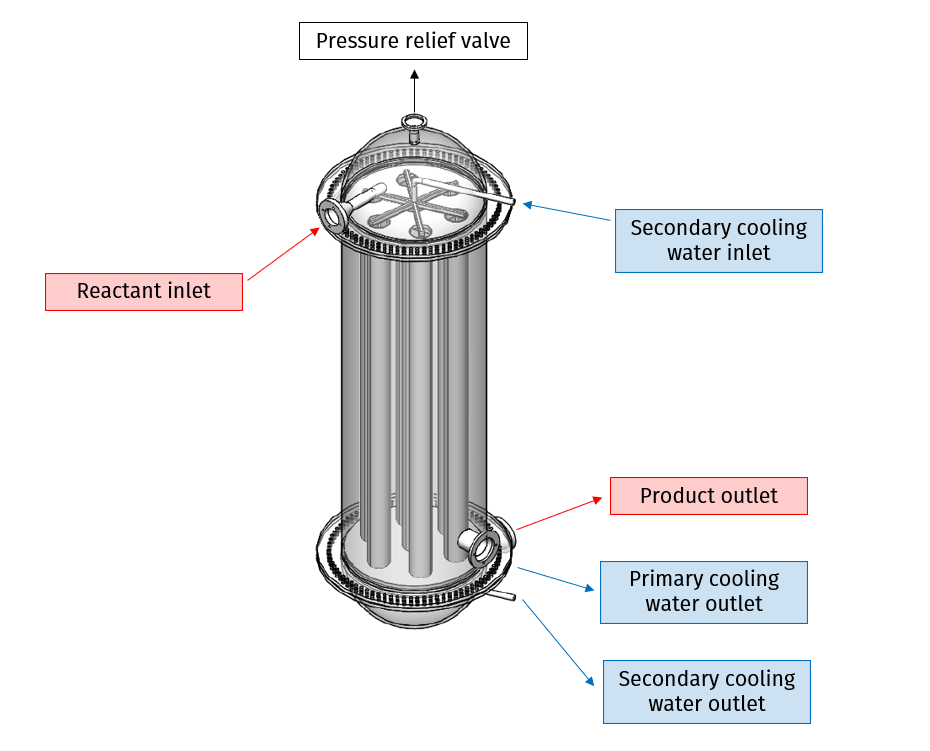
\includegraphics[width=\linewidth]{chapters/0-executive-summary/figures/FYD executive sum.PNG}
    \caption{Mechanical design of Nitroma's nitration reactor}
    \label{fig:executivesummaryreactor}
\end{wrapfigure}
A key aspect of innovation in the nitration reactor is its ability to have a robust temperature control within its compact design. This was achieved by having a state-of-the-art triple concentric tube arrangement. Each of the 7 reaction tubes are surrounded by an outer primary cooling water jacket, with an additional secondary concentric pipe through the centre of each reaction tube. The reactor is also packed with a highly thermally conductive Silicon Carbide foam to immobilise the H-mordenite catalyst. By combining these features together, the HEX reactor keeps the temperature of the exothermic reaction below the safe limit of 363K, while ensuring that > 98\% conversion is achieved within the reactor length.
The reactor material chosen is stainless steel 304L, which is suitable for corrosive nitric acid processing (). The wall thickness of the shell and ends were calculated to be 5mm after taking into consideration of corrosion and other welding factors. The final reactor design can be seen in Figure \ref{fig:executivesummaryreactor}

%kinetics and modelling approach [andreas]
The kinetics of the zeolite-catalysed nitration reaction were determined using literature data and the Arrhenius equation. To allow for more accurate modelling, the rate equation for the production of each nitrotoluene isomer were determined. 

The model was implemented and optimised on COMSOL 5.6. 
- general model used (porous media) and show 1 comsol plot to get Ali excited
- prevent hotspot thermal runaway etc

%optimisation [zong]
To ensure the reactor operates in optimal conditions, the following parameters were optimised and used in the final reactor design: Concentric inner cooling pipe diameter and flowrate, direction of cooling water flow, \ch{HNO3} to toluene inlet ratio and the total number of reaction tubes. %A further sensitivity analysis was performed on the cooling water inlet temperature since the temperature inside the reactor needs to be well-controlled at all times. Cooling water temperature was simulated to vary by \pm 5 K and the total length of reactor required was investigated. The cooling water is not expected to fluctuate to this degree since it is reused and mixed together from multiple cooling water streams in the plant, but taking a conservative approach to model the reactor increases the overall safety of Nitroma's plant in the worst case scenario. 
The optimal reactor length was determined to be 4.2m. 


%mech design [loon]
